\chapter{Persistence}
\section{Aims}
\paragraph{} At the end of the practical portion of this topic you will be able to:

\begin{itemize}
\item Use Shared Preferences to store basic Java datatypes in Key:Value format
\item Use Internal \& external storage to store files
\item Use SQLite to store data in Android's default DB system
\end{itemize}

\section{Shared Preferences}
\paragraph{} Shared preferences (accessed through the SharedPreferences class) are a dictionary of key-value pairs that can be used to store primitive Java data-types. This is most commonly used to store app and user settings and preferences or small amounts of simple data. 

\paragraph{} Using shared preferences to store small bits of data, confined to basic Java datatypes, is straightforward. Lets try it out now.  We are going to create an app that displays two buttons. One button will store some data, a randomly generated high score, in our shared preferences and the other button will read some data from our shared preferences. To keep things simple, feedback of what is read or written will be displayed after each button press using Toasts. This small app will illustrate how to store a single key and value into a specified shared preferences file. You should be able to build on this to incorporate simple data storage of Java datatypes into your app if appropriate.

\paragraph{} Create a new Android project and delete the `Hello World' label. Now open `strings.xml' and add some new strings. We need a string to store the name of the shared preferences file `preference\_file\_name' and a string for the name of our data key `high\_score'. We also need two more strings for the labels for our buttons, `get\_something' and `do\_something'. Our strings.xml should look similar to this:

\begin{lstlisting}
<resources>
    <string name="app_name">SharedPreferences</string>
    <string name="preference_file_name">MyPrefs</string>
    <string name="high_score">0</string>
    <string name="get_something">Get Prefs</string>
    <string name="do_something">Add Pref</string>
</resources>
\end{lstlisting}

\paragraph{} Now we can edit our layout to display the buttons. Edit your activity\_main.xml so that it uses a LinearLayout and give this layout two buttons, `btn1' and `btn2' as children. The text for `btn1' should use the `get\_something' string and the text for `btn2' should use the `do\_something' string that we just added to strings.xml. When you are done, your activity\_main.xml should look something like this:

\begin{lstlisting}
<?xml version="1.0" encoding="utf-8"?>
<LinearLayout xmlns:android="http://schemas.android.com/apk/res/android"
    xmlns:tools="http://schemas.android.com/tools"
    android:id="@+id/activity_main"
    android:layout_width="match_parent"
    android:layout_height="match_parent"
    android:paddingBottom="@dimen/activity_vertical_margin"
    android:paddingLeft="@dimen/activity_horizontal_margin"
    android:paddingRight="@dimen/activity_horizontal_margin"
    android:paddingTop="@dimen/activity_vertical_margin"
    android:orientation="vertical"
    tools:context="org.simonwells.sharedpreferences.MainActivity">

    <Button
        android:layout_width="wrap_content"
        android:layout_height="wrap_content"
        android:text="@string/get_something"
        android:id="@+id/btn1"
        android:layout_gravity="center_horizontal" />

    <Button
        android:layout_width="wrap_content"
        android:layout_height="wrap_content"
        android:text="@string/do_something"
        android:id="@+id/btn2"
        android:layout_gravity="center_horizontal" />

</LinearLayout>
\end{lstlisting}

\paragraph{} Ensure that your app compiles and runs before proceeding. If necessary, fix any bugs or typos as there's no point adding more code until what we have works. Our MainActivity.java file should end up looking something similar to the following:

\begin{lstlisting}
package org.simonwells.sharedpreferences;

import android.content.Context;
import android.content.SharedPreferences;
import android.support.v7.app.AppCompatActivity;
import android.os.Bundle;
import android.view.View;
import android.widget.Button;
import android.widget.Toast;

import java.util.Map;
import java.util.Random;

public class MainActivity extends AppCompatActivity {

    @Override
    protected void onCreate(Bundle savedInstanceState) {
        super.onCreate(savedInstanceState);
        setContentView(R.layout.activity_main);

        final Random rnd = new Random();

        Button get_something = (Button) findViewById(R.id.btn1);
        get_something.setOnClickListener(new View.OnClickListener() {
            @Override
            public void onClick(View view) {
                SharedPreferences prefs = getBaseContext().getSharedPreferences("MyPrefs", Context.MODE_PRIVATE);
                Map mp = prefs.getAll();
                Toast.makeText(getBaseContext(), mp.toString(), Toast.LENGTH_SHORT).show();
            }
        });

        Button do_something = (Button) findViewById(R.id.btn2);
        do_something.setOnClickListener(new View.OnClickListener() {
            @Override
            public void onClick(View view) {
                SharedPreferences prefs = getBaseContext().getSharedPreferences("MyPrefs", Context.MODE_PRIVATE);
                int newHighScore = rnd.nextInt(1000);
                SharedPreferences.Editor editor = prefs.edit();
                editor.putInt("0", newHighScore);
                editor.commit();
                Toast.makeText(getBaseContext(), "New High Score: "+newHighScore, Toast.LENGTH_SHORT).show();
            }
        });
    }
}
\end{lstlisting}

\paragraph{} Let's take a look at all the things that we just did:

\begin{enumerate}
\item Set up a random number object, e.g.
\begin{lstlisting}
    final Random rnd = new Random();
\end{lstlisting}
\item Create a button handler to retrieve all of the keys and values in the shared preference file as a map and display the contents of the map in a Toast.
\begin{lstlisting}
Button get_something = (Button) findViewById(R.id.btn1);
        get_something.setOnClickListener(new View.OnClickListener() {
            @Override
            public void onClick(View v) {
                SharedPreferences prefs = getBaseContext().getSharedPreferences(getString(R.string.preference_file_name), Context.MODE_PRIVATE);
                Map mp = prefs.getAll();
                Toast.makeText(getBaseContext(), mp.toString(), Toast.LENGTH_SHORT).show();
            }
        });
\end{lstlisting}
\item Create a button handler in which we edit our shared preference file to set a high score value, basically store an int that our random number object supplies.
\begin{lstlisting}
Button do_something = (Button) findViewById(R.id.btn2);
        do_something.setOnClickListener(new View.OnClickListener() {
            @Override
            public void onClick(View v) {
                SharedPreferences prefs = getBaseContext().getSharedPreferences(getString(R.string.preference_file_name), Context.MODE_PRIVATE);
                //Map mp = prefs.getAll();
                int newHighScore = rnd.nextInt(1000);
                SharedPreferences.Editor editor = prefs.edit();
                editor.putInt(getString(R.string.high_score), newHighScore);
                editor.commit();
                Toast.makeText(getBaseContext(), "New High Score"+newHighScore, Toast.LENGTH_SHORT).show();
            }
        });
\end{lstlisting}
\end{enumerate}


\paragraph{} When you run it, your new app should look something like the following:

\begin{figure}[H]
\centering
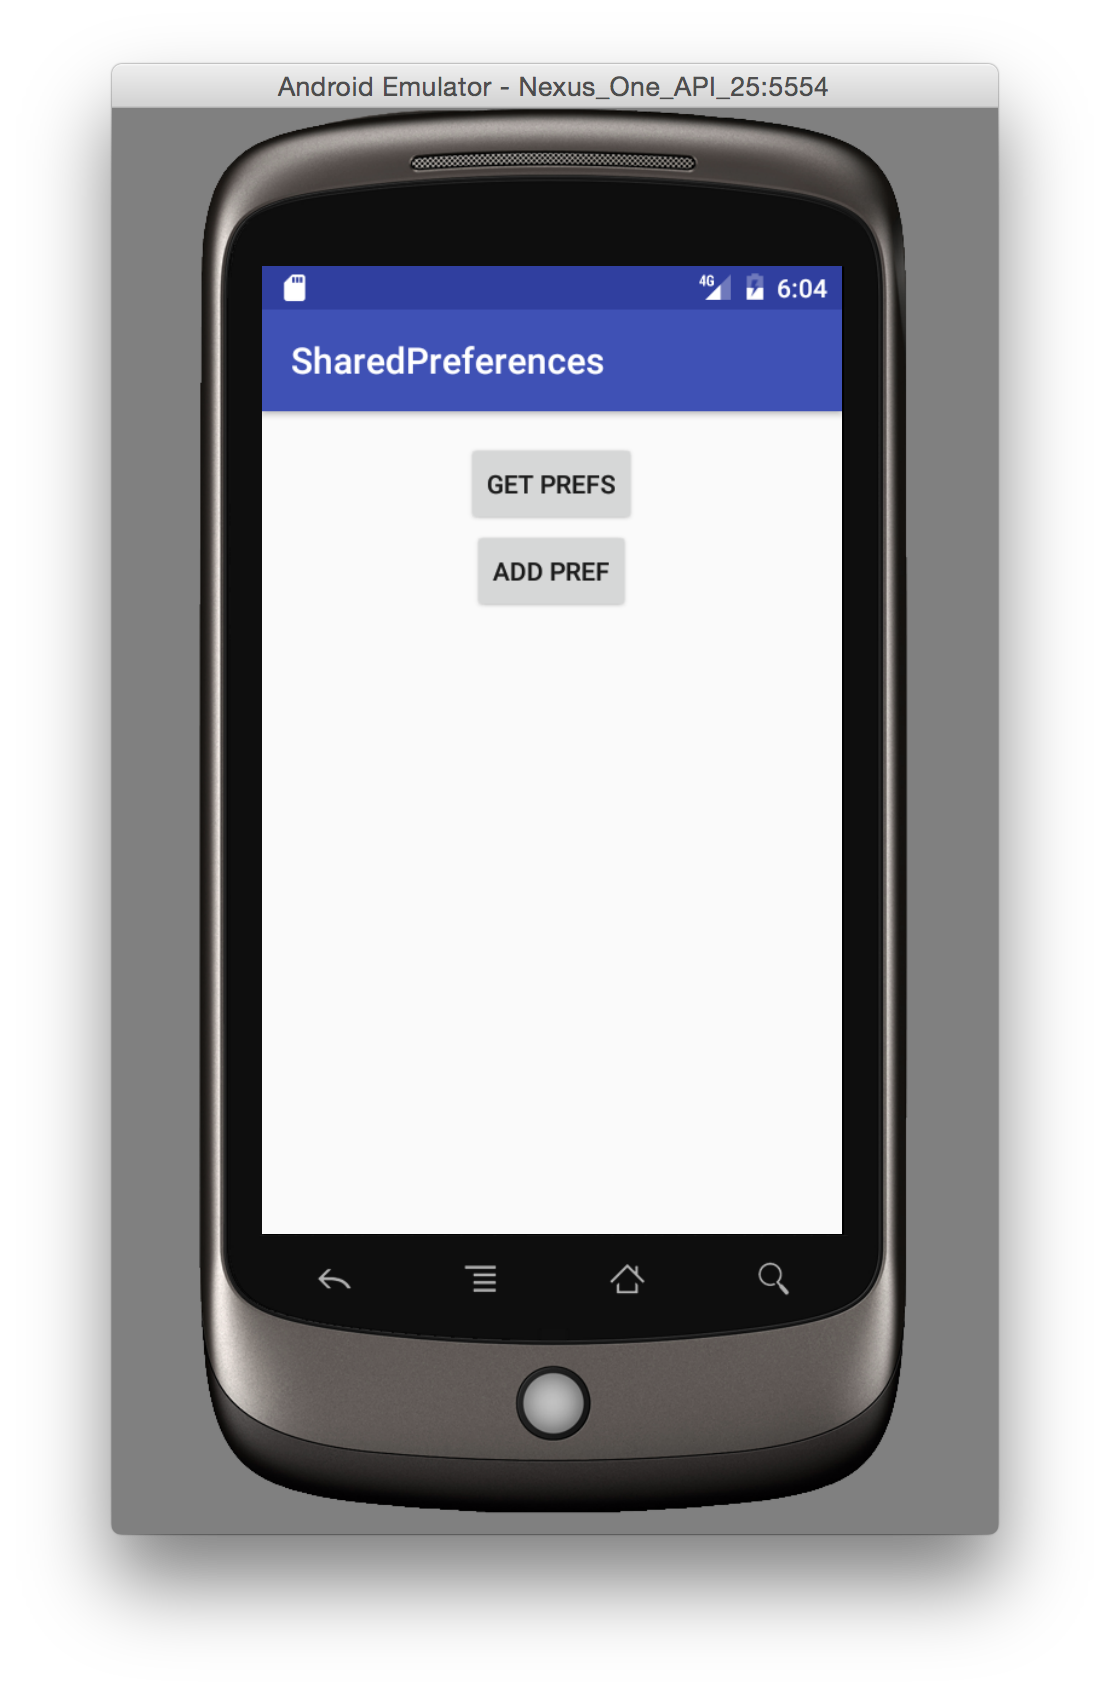
\includegraphics[width=0.8\textwidth]{images/sharedprefs_avd}
\caption{The Shared Prefs Example}
\label{fig:sharedprefs_avd}
\end{figure}

\paragraph{} You should use the Shared preferences documentation\footnote{\url{http://developer.android.com/reference/android/content/SharedPreferences.html}} to explore more functionality of this aspect of data storage. Try retrieving the specific key rather than all of the keys in the get\_something button handler. Now try storing your name into the shared preferenced file and retrieving it.

\paragraph{} Although you can exploit this for more advanced data storage requirements, the trouble and complexities of doing so can mean that it is better to adopt other strategies. The most appropriate storage method for a given app is highly dependent upon that app, what it is designed to do, and how that design is implemented.

\section{Internal Storage}
\paragraph{} Every app has a private directory, outside of the application bundle, in which it can store files. This is usually located on the devices internal storage and is private to the app and cannot be accessed by any other apps. These files are tied to the lifetime of the app and deleted when the app is deleted (but are kept during updates). The Android training documentation\footnote{\url{http://developer.android.com/training/basics/data-storage/files.html}} has more information on saving files to internal storage.

\paragraph{} For this part of the pracical we will build a similar interface to the one we did for the shared preferences data perisistence example earlier, e.g. a button to save some data to a file on internal storage and a button to load the data from that file and display the loaded data using a Toast. The data we will store will be the data as this is something that is straightforward to generate and is dynamic so will change the data stored each time we press the save button.

\paragraph{} Create a new Android project. Delete the `Hello World' TextView and add to buttons, `Save Something' and `load something' to a vertical LinearLayout. Add appropriate strings to support this to strings.xml so that your activity\_main.xml i something like the following:

\begin{lstlisting}
<RelativeLayout xmlns:android="http://schemas.android.com/apk/res/android"
    xmlns:tools="http://schemas.android.com/tools" android:layout_width="match_parent"
    android:layout_height="match_parent" android:paddingLeft="@dimen/activity_horizontal_margin"
    android:paddingRight="@dimen/activity_horizontal_margin"
    android:paddingTop="@dimen/activity_vertical_margin"
    android:paddingBottom="@dimen/activity_vertical_margin" tools:context=".MainActivity">

    <LinearLayout
        android:orientation="vertical"
        android:layout_width="fill_parent"
        android:layout_height="fill_parent"
        android:layout_centerVertical="true"
        android:layout_centerHorizontal="true">

        <Button
            android:layout_width="wrap_content"
            android:layout_height="wrap_content"
            android:text="@string/save_file"
            android:id="@+id/button1"
            android:layout_gravity="center_horizontal" />

        <Button
            android:layout_width="wrap_content"
            android:layout_height="wrap_content"
            android:text="@string/load_file"
            android:id="@+id/button2"
            android:layout_gravity="center_horizontal" />
    </LinearLayout>
</RelativeLayout>
\end{lstlisting}

\paragraph{} and your strings.xml is something like the following:

\begin{lstlisting}
<?xml version="1.0" encoding="utf-8"?>
<resources>

    <string name="app_name">TestInternalFile</string>
    <string name="hello_world">Hello world!</string>
    <string name="action_settings">Settings</string>
    <string name="load_file">LOAD SOMETHING</string>
    <string name="save_file">SAVE SOMETHING</string>

</resources>
\end{lstlisting}

\paragraph{} That gives us an interface with some buttons ready to do something. Now all we need to do is get the buttons to actually do something, like saving and loading files. To do this we need to add click listeners for each button to the onCreate method in MainActivity.java where the listener for the first button creates a new file, generates a string from the current date, then writes the string to the file we specified. For example, 

\begin{lstlisting}
Button btn1 = (Button) findViewById(R.id.button1);
        btn1.setOnClickListener(new View.OnClickListener() {
            @Override
            public void onClick(View v) {

                String filename = "napierfile";
                String outString = new Date().toString();
                FileOutputStream outStream;

                try {
                    outStream = getApplicationContext().openFileOutput(filename, Context.MODE_PRIVATE);
                    outStream.write(outString.getBytes());
                    outStream.close();
                } catch (Exception e) {
                    e.printStackTrace();
                }
            }
        });
\end{lstlisting}

\paragraph{} For our second button we want to read in the contents of our specified file then display those contents in a Toast. For example,

\begin{lstlisting}
Button btn2 = (Button) findViewById(R.id.button2);
        btn2.setOnClickListener(new View.OnClickListener() {
            @Override
            public void onClick(View v) {
                int ch;

                String filename = "napierfile";
                StringBuffer inString = new StringBuffer("");
                FileInputStream inStream;

                try {
                    inStream = getApplicationContext().openFileInput(filename);
                    try {
                        while ((ch = inStream.read()) != -1)
                            inString.append((char) ch);
                    } catch (IOException e) {
                        e.printStackTrace();
                    }
                    inStream.close();
                } catch (Exception e) {
                    e.printStackTrace();
                }

                String data = new String(inString);
                Toast.makeText(getBaseContext(),data,Toast.LENGTH_SHORT).show();
            }
        });
\end{lstlisting}

\paragraph{} Putting this all together, our MainActivity.java should look something similar to the following:

\begin{lstlisting}
package org.simonwells.testinternalfile;

import android.content.Context;
import android.support.v7.app.ActionBarActivity;
import android.os.Bundle;
import android.view.Menu;
import android.view.MenuItem;
import android.view.View;
import android.widget.Button;
import android.widget.Toast;

import java.io.FileInputStream;
import java.io.FileOutputStream;
import java.io.IOException;
import java.util.Date;


public class MainActivity extends ActionBarActivity {

    @Override
    protected void onCreate(Bundle savedInstanceState) {
        super.onCreate(savedInstanceState);
        setContentView(R.layout.activity_main);

        Button btn1 = (Button) findViewById(R.id.button1);
        btn1.setOnClickListener(new View.OnClickListener() {
            @Override
            public void onClick(View v) {

                String filename = "napierfile";
                String outString = new Date().toString();
                FileOutputStream outStream;

                try {
                    outStream = getApplicationContext().openFileOutput(filename, Context.MODE_PRIVATE);
                    outStream.write(outString.getBytes());
                    outStream.close();
                } catch (Exception e) {
                    e.printStackTrace();
                }
            }
        });

        Button btn2 = (Button) findViewById(R.id.button2);
        btn2.setOnClickListener(new View.OnClickListener() {
            @Override
            public void onClick(View v) {
                int ch;

                String filename = "napierfile";
                StringBuffer inString = new StringBuffer("");
                FileInputStream inStream;

                try {
                    inStream = getApplicationContext().openFileInput(filename);
                    try {
                        while ((ch = inStream.read()) != -1)
                            inString.append((char) ch);
                    } catch (IOException e) {
                        e.printStackTrace();
                    }
                    inStream.close();
                } catch (Exception e) {
                    e.printStackTrace();
                }

                String data = new String(inString);
                Toast.makeText(getBaseContext(),data,Toast.LENGTH_SHORT).show();
            }
        });
    }

    @Override
    public boolean onCreateOptionsMenu(Menu menu) {
        // Inflate the menu; this adds items to the action bar if it is present.
        getMenuInflater().inflate(R.menu.menu_main, menu);
        return true;
    }

    @Override
    public boolean onOptionsItemSelected(MenuItem item) {
        // Handle action bar item clicks here. The action bar will
        // automatically handle clicks on the Home/Up button, so long
        // as you specify a parent activity in AndroidManifest.xml.
        int id = item.getItemId();

        //noinspection SimplifiableIfStatement
        if (id == R.id.action_settings) {
            return true;
        }

        return super.onOptionsItemSelected(item);
    }
}
\end{lstlisting}

\section{Internal Storage: Caching}
\paragraph{} Android provides a mechanism for caching files which can be used for temporary storage that need not be kept for ever. For example, if you build a navigation app that uses maps you might want to cache lots of map files for the area that your user is in to enable a good and responsive experience. However, map data uses a lot of storage, and can usually be re-downloaded as requiredso you might plan to use the cache directory to store mapping data so that, if the device begins to run low on storage, the Android OS can reclaim storage space by emptying the cache. Notice that this is an {\emph{emergency measure}} - you must still maintain the size of data that you use as small and current so that you do not waste resources as the OS does not empty the cache periodically but only when storage space needs to be reclaimed in order to ensure reliable overall system functionality. You should also take not that users can also manually clear the cache at any time.

\paragraph{} If you are caching data to storage from your app, and it is fine for the OS to delete that data {\bf{at any time}} then the cache is a good place to store it.

\section{External Storage}
\paragraph{} External storage is basically any storage on the device that is public to all apps, but this term usually refers to SD card storage or USB storage. NB. Occasionally the internal storage hardware of a device might be partitioned to provide both internal (private) and external (public) storage. In this case such storage can be accessed as normal.

\paragraph{} To use external storage we need to edit your apps manifest file to enable the app to obtain permission. For example, within your app's AndroidManifest.xml file:

\begin{lstlisting}
<manifest ...>
    <uses-permission android:name="android.permission.WRITE_EXTERNAL_STORAGE" />
    ...
</manifest>
\end{lstlisting}

\paragraph{} Working with files on external storage is very similar to the example for internal storage except that, because external storage might not be available, for example, you might remove the SD card, you need to do some checks first. For example, to check if external storage is available to read and write we could use a code fragment like this:

\begin{lstlisting}
String state = Environment.getExternalStorageState();
if (Environment.MEDIA_MOUNTED.equals(state)) {
    
    // Code for creating, reading, writing file as for
    // working with internal storage

}
\end{lstlisting}

\paragraph{} We also need to use a different method to retrieve a path to the external files directory as shown in this code fragment:

\begin{lstlisting}
File file = new File(getApplicationContext().getExternalFilesDir(null), "napier.txt");
\end{lstlisting}

\paragraph{} Lets quickly put together an app that saves data to external storage and loads it, again using a button to load, a button to save, and a Toast to display the loaded data. This will involve editing the following files:

\begin{itemize}
\item strings.xml
\item activity\_main.xml
\item AndroidManifest.xml
\item MainActivity.java
\end{itemize}

\paragraph{} So lets get started. Set up your Activity to hold a user interface displaying two buttons as we did for the internal storage. You should have an activity\_main.xml that looks similar to this:

\begin{lstlisting}
<RelativeLayout xmlns:android="http://schemas.android.com/apk/res/android"
    xmlns:tools="http://schemas.android.com/tools" android:layout_width="match_parent"
    android:layout_height="match_parent" android:paddingLeft="@dimen/activity_horizontal_margin"
    android:paddingRight="@dimen/activity_horizontal_margin"
    android:paddingTop="@dimen/activity_vertical_margin"
    android:paddingBottom="@dimen/activity_vertical_margin" tools:context=".MainActivity">

    <LinearLayout
        android:orientation="vertical"
        android:layout_width="fill_parent"
        android:layout_height="fill_parent"
        android:layout_centerHorizontal="true"
        android:layout_alignParentTop="true">

        <Button
            android:layout_width="wrap_content"
            android:layout_height="wrap_content"
            android:text="@string/save_file"
            android:id="@+id/button1"
            android:layout_gravity="center_horizontal" />

        <Button
            android:layout_width="wrap_content"
            android:layout_height="wrap_content"
            android:text="@string/load_file"
            android:id="@+id/button2"
            android:layout_gravity="center_horizontal" />
    </LinearLayout>
</RelativeLayout>

\end{lstlisting}

\paragraph{} and a strings.xml that looks similar to this:

\begin{lstlisting}
<?xml version="1.0" encoding="utf-8"?>
<resources>

    <string name="app_name">TestExternalFile</string>
    <string name="hello_world">Hello world!</string>
    <string name="action_settings">Settings</string>
    <string name="save_file">SAVE</string>
    <string name="load_file">LOAD</string>

</resources>
\end{lstlisting}

\paragraph{} Now add the permission line to your AndroidManifest.xml so that we can use external storage. That file should look something like this:

\begin{lstlisting}
<?xml version="1.0" encoding="utf-8"?>
<manifest xmlns:android="http://schemas.android.com/apk/res/android"
    package="org.simonwells.testexternalfile" >

    <application
        android:allowBackup="true"
        android:icon="@drawable/ic_launcher"
        android:label="@string/app_name"
        android:theme="@style/AppTheme" >
        <activity
            android:name=".MainActivity"
            android:label="@string/app_name" >
            <intent-filter>
                <action android:name="android.intent.action.MAIN" />

                <category android:name="android.intent.category.LAUNCHER" />
            </intent-filter>
        </activity>
    </application>

    <uses-permission android:name="android.permission.WRITE_EXTERNAL_STORAGE"/>

</manifest>

\end{lstlisting}

\paragraph{} Now we can use some java to glue everything together. We need click handlers for each of the load and save buttons as shown here:

\begin{lstlisting}
package org.simonwells.testexternalfile;

import android.os.Environment;
import android.support.v7.app.ActionBarActivity;
import android.os.Bundle;
import android.view.Menu;
import android.view.MenuItem;
import android.view.View;
import android.widget.Button;
import android.widget.Toast;

import java.io.File;
import java.io.FileInputStream;
import java.io.FileOutputStream;
import java.io.IOException;
import java.io.InputStream;
import java.io.OutputStream;
import java.util.Date;


public class MainActivity extends ActionBarActivity {

    @Override
    protected void onCreate(Bundle savedInstanceState) {
        super.onCreate(savedInstanceState);
        setContentView(R.layout.activity_main);

        Button btn1 = (Button) findViewById(R.id.button1);
        btn1.setOnClickListener(new View.OnClickListener() {
            @Override
            public void onClick(View v) {
                String state = Environment.getExternalStorageState();
                if (Environment.MEDIA_MOUNTED.equals(state)) {
                    File file = new File(getApplicationContext().getExternalFilesDir(null), "napier.txt");
                    String datetime = new Date().toString();

                    try{
                        OutputStream os = new FileOutputStream(file);
                        os.write(datetime.getBytes());
                        os.close();
                    } catch(Exception e){ e.printStackTrace(); }
                }
            }
        });

        Button btn2 = (Button) findViewById(R.id.button2);
        btn2.setOnClickListener(new View.OnClickListener() {
            @Override
            public void onClick(View v) {
                String state = Environment.getExternalStorageState();
                if (Environment.MEDIA_MOUNTED.equals(state)){
                    File file = new File(getApplicationContext().getExternalFilesDir(null), "napier.txt");
                    StringBuffer inStr = new StringBuffer("");
                    int ch;

                    try{
                        InputStream is = new FileInputStream(file);
                        while ((ch = is.read()) != -1){
                            inStr.append((char) ch);
                        }
                        is.close();
                    } catch(IOException e) { e.printStackTrace(); }
                    String data = new String(inStr);
                    Toast.makeText(getApplicationContext(), data, Toast.LENGTH_SHORT).show();
                }
            }
        });
    }


    @Override
    public boolean onCreateOptionsMenu(Menu menu) {
        // Inflate the menu; this adds items to the action bar if it is present.
        getMenuInflater().inflate(R.menu.menu_main, menu);
        return true;
    }

    @Override
    public boolean onOptionsItemSelected(MenuItem item) {
        // Handle action bar item clicks here. The action bar will
        // automatically handle clicks on the Home/Up button, so long
        // as you specify a parent activity in AndroidManifest.xml.
        int id = item.getItemId();

        //noinspection SimplifiableIfStatement
        if (id == R.id.action_settings) {
            return true;
        }

        return super.onOptionsItemSelected(item);
    }
}
\end{lstlisting}

\paragraph{} We can now double check that the file is stored on the external storage. On your Android device, or in the emulator, open the `My files' app and click on `Android' then `data'. Now find the folder that matches the namespace for your app, e.g. starting uk.ac.napier or whatever you used when you set up the Android project. Within that folder you should select `files' and you should then be presented with `napier.txt'. Clicking on this file should bring up an intent selection dialogue so that you can decide which app to open it in. Select an app and you should see the datetime string displayed from the last time you used your app to store a file to external storage.

\paragraph{} There are a few things to consider when storing data on external storage. For example, many app can scan external storage, because it is public, to find music, ringtones, videos, picture, \&c. If you don't want, for example an MP3, to show up on such a scan then creating an empty file called .nomedia in the directory holding the MP3 will cause that folder to be ignored by media scanners. Similarly, if your app scans externl storage for media files to use then it should also respect the .nomedia convention and ignore any directories containing a file so-named. In contrast however, if you do want to share media from your app with other apps then you should consider using the default directories such as Music/, Ringtones/, \&c. to store those files as this is the expected location for them and the places that users will look to find such files.

\section{SQLite}
\paragraph{} Using SQLite is a common exercise on Android for storing data. There are many tutorials onlinethat describe the initial setup required but most of this is actually using Java rather than an Android topic so using SQLite in Android is left as an advanced exercise for now. If you have done the other persistence exercises earlier in the chapter then you should research SQLite on Android and work through some online tutorials.

